\documentclass[10pt]{exam}

\usepackage{amssymb, amsmath, amsthm, mathrsfs, multicol, graphicx}
\usepackage{tikz}

 \def\d{\displaystyle}
\def\?{\reflectbox{?}}
\def\b#1{\mathbf{#1}}
\def\f#1{\mathfrak #1}
\def\c#1{\mathcal #1}
\def\s#1{\mathscr #1}
\def\r#1{\mathrm{#1}}
\def\N{\mathbb N}
\def\Z{\mathbb Z}
\def\Q{\mathbb Q}
\def\R{\mathbb R}
\def\C{\mathbb C}
\def\F{\mathbb F}
\def\A{\mathbb A}
\def\X{\mathbb X}
\def\E{\mathbb E}
\def\O{\mathbb O}
\def\U{\mathcal U}
\def\pow{\mathcal P}
\def\inv{^{-1}}
\def\nrml{\triangleleft}
\def\st{:}
\def\~{\widetilde}
\def\rem{\mathcal R}
\def\sigalg{$\sigma$-algebra }
\def\Gal{\mbox{Gal}}
\def\iff{\leftrightarrow}
\def\Iff{\Leftrightarrow}
\def\land{\wedge}
\def\And{\bigwedge}
\def\AAnd{\d\bigwedge\mkern-18mu\bigwedge}
\def\Vee{\bigvee}
\def\VVee{\d\Vee\mkern-18mu\Vee}
\def\imp{\rightarrow}
\def\Imp{\Rightarrow}
\def\Fi{\Leftarrow}

%\def\={\equiv}
\def\var{\mbox{var}}
\def\mod{\mbox{Mod}}
\def\Th{\mbox{Th}}
\def\sat{\mbox{Sat}}
\def\con{\mbox{Con}}
\def\bmodels{=\joinrel\mathrel|}
\def\iffmodels{\bmodels\models}
\def\dbland{\bigwedge \!\!\bigwedge}
\def\dom{\mbox{dom}}
\def\rng{\mbox{range}}
\DeclareMathOperator{\wgt}{wgt}


\def\bar{\overline}


\newcommand{\vtx}[2]{node[fill,circle,inner sep=0pt, minimum size=4pt,label=#1:#2]{}}
\newcommand{\va}[1]{\vtx{above}{#1}}
\newcommand{\vb}[1]{\vtx{below}{#1}}
\newcommand{\vr}[1]{\vtx{right}{#1}}
\newcommand{\vl}[1]{\vtx{left}{#1}}
\renewcommand{\v}{\vtx{above}{}}

\def\circleA{(-.5,0) circle (1)}
\def\circleAlabel{(-1.5,.6) node[above]{$A$}}
\def\circleB{(.5,0) circle (1)}
\def\circleBlabel{(1.5,.6) node[above]{$B$}}
\def\circleC{(0,-1) circle (1)}
\def\circleClabel{(.5,-2) node[right]{$C$}}
\def\twosetbox{(-2,-1.4) rectangle (2,1.4)}
\def\threesetbox{(-2.5,-2.4) rectangle (2.5,1.4)}
\newcommand{\twoline}[2]{\begin{pmatrix}#1 \\ #2 \end{pmatrix}}


\def\circleA{(-.5,0) circle (1)}
\def\circleAlabel{(-1.5,.6) node[above]{$A$}}
\def\circleB{(.5,0) circle (1)}
\def\circleBlabel{(1.5,.6) node[above]{$B$}}
\def\circleC{(0,-1) circle (1)}
\def\circleClabel{(.5,-2) node[right]{$C$}}
\def\twosetbox{(-2,-1.5) rectangle (2,1.5)}
\def\threesetbox{(-2,-2.5) rectangle (2,1.5)}


%\pointname{pts}
\pointsinmargin
\marginpointname{pts}
\marginbonuspointname{pts-bns}
\addpoints
\pagestyle{head}
\printanswers

\firstpageheader{Math 228}{\textbf{Homework 3}}{Due: September 12}


\begin{document}
\noindent \textbf{Instructions}: Same rules as usual.  Write up solutions on separate sheets of paper; you may work together to understand the problems, but write up your solutions individually.  You may NOT look for solutions online or in other books.

\begin{questions}



\question[6] A \emph{Hamilton path} is a walk that visits every vertex exactly once.  A \emph{Hamilton cycle} is is a Hamilton path that starts and stops at the same vertex (it is okay that the starting/stopping vertex is visited twice, but no other vertex may be).  Consider the following graph:

\begin{center}
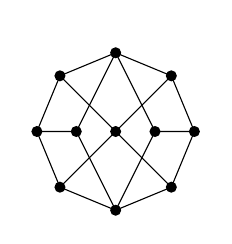
\begin{tikzpicture}[scale=.5]
\foreach \x in {0, 45, ..., 315}
  \draw  (\x:2) \v -- (\x+45:2);
\draw (0,0) \v -- (45:2) (0,0) -- (135:2) (0,0) -- (225:2) (0,0) -- (315:2);
\draw (-1,0) \v -- (90:2) (-1,0) -- (180:2) (-1,0) -- (270:2);
\draw (1,0) \v -- (90:2) (1,0) -- (0:2) (1,0) -- (270:2);
\end{tikzpicture}
\end{center}

\begin{parts}
	\part Find a Hamilton path.  Can your path be extended to a Hamilton cycle?
	\part Is the graph bipartite?  If so, partition the vertices into two parts $X$ and $Y$ and say how many vertices are in each ``part''?
	\part Use your answer to part (b) to prove that the graph has \underline{no} Hamilton \emph{cycle}.
\end{parts}

\begin{solution}
  \begin{parts}
    \part One path is shown below:

    \begin{center}
    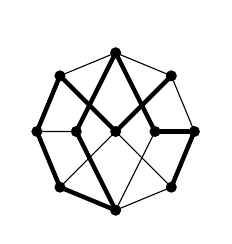
\begin{tikzpicture}[scale=.5]
    \foreach \x in {0, 45, ..., 315}
      \draw  (\x:2) \v -- (\x+45:2);
    \draw (0,0) \v -- (45:2) (0,0) -- (135:2) (0,0) -- (225:2) (0,0) -- (315:2);
    \draw (-1,0) \v -- (90:2) (-1,0) -- (180:2) (-1,0) -- (270:2);
    \draw (1,0) \v -- (90:2) (1,0) -- (0:2) (1,0) -- (270:2);
    \draw[ultra thick] (45:2) -- (0,0);
    \draw[ultra thick] (0,0) -- (135:2);
    \draw[ultra thick] (135:2) -- (180:2);
    \draw[ultra thick] (180:2) -- (225:2);
    \draw[ultra thick] (225:2) -- (270:2);
    \draw[ultra thick] (270:2) -- (-1,0);
    \draw[ultra thick] (-1,0) -- (0,2);
    \draw[ultra thick] (0,2) -- (1,0);
    \draw[ultra thick] (1,0) -- (2,0);
    \draw[ultra thick] (2,0) -- (315:2);
    \end{tikzpicture}
    \end{center}
    This path cannot be extended to a cycle (none could be, as seen below).
    \part Yes, the graph is bipartite. Partitioning the vertices into sets $A$ and $B$ will always gives one set 5 vertices and the other 6.
    \part Notice that any Hamilton path (or cycle) must alternate between sides/sets of the bipartite graph.  To have a path, we must start at one of the vertices on the larger side, but then after visiting all 11 vertices, we will be back on the larger side, so we will not be able to travel to the starting vertex (which is a different vertex on the same side).  In general, this says that if a bipartite graph has a Hamilton cycle, then the two sides of the bipartite graph must have the same size.
  \end{parts}
\end{solution}


\question[6] Suppose $G$ is a bipartite graph with parts $A$ and $B$.  Consider the statement: If one part of $G$ has at least two more vertices than the other, then $G$ does not have a Hamilton path.

\begin{parts}
	\part Write the converse, contrapositive, and negation of the statement.
	\part Prove the statement is true.  Clearly identity what style of proof (direct, contrapositive, or contradiction) you use.
\end{parts}

\begin{solution}
  \begin{parts}
    \part The converse: If $G$ does not have a Hamilton path, then one part of $G$ has at least two more vertices than the other.

    Contrapositive: If $G$ does have a Hamilton path, then neither part of $G$ has more than one vertex more than the other.

    Negation: One part of $G$ has at least two more vertices than the other, and $G$ has a Hamilton path.

    \part We will use a proof by contrapositive (a proof by contradiction would also work).

    Suppose $G$ has a Hamilton path, say $v_1, v_2, v_3, \ldots, v_n$ (where $n$ is the number of vertices in $G$).  Now $v_1$ must not be in the same part as $v_2$, since there cannot be edges between vertices in the same part.  Similarly, $v_3$ cannot be in the same part as $v_2$, and thus must be in the same part as $v_1$.  Continuing in this way, we see that $v_{2i}$ must all be in the same part, and $v_{2i+1}$ must all be in the other part, for all $i$.

    Either $n$ is even or odd.  If $n$ is even, this says that the two parts must have the same size.  If $n$ is odd, then $v_n$ is in the same part as $v_1$, and then there will be one more vertex in this part than the other.
  \end{parts}

\end{solution}

\question[4] Consider graphs with $n$ vertices.  Remember, graphs do not need to be \emph{connected}.  You might want to try to answer the following questions for some specific values of $n$ to get a feel for them, but your final answers should be in terms of $n$.
\begin{parts}
  \part How many edges must the graph have to guarantee at least one vertex has degree 2 or more?  Prove your answer.
  \part How many edges must the graph have to guarantee all vertices have degree 2 or more?  Prove your answer.
\end{parts}

\begin{solution}
  \begin{parts}
    \part Note that if $n$ is even, it would be possible to draw a graph with $n/2$ edges where each vertex has degree 1.  If $n$ is odd, then $\lfloor n/2\rfloor$ (that is, $n/2$ rounded down) has this property.

    We will prove that if a graph with $n$ vertices has more than $n/2$ edges, there must be a vertex of degree 2 or higher.  The proof will be by contrapositive.  Assume a graph with $n$ vertices has every vertex with degree at most 1.  Then there are at most $n/2$ edges (since the number of edges is twice the sum of the degrees).  That completes the proof.

    \part How could a graph not have the property that all vertices have degree two or more?  This could happen if one vertex has degree 1, and all the other have high degree.  The largest degree the remaining vertices could have would be $n-2$, except for one that has degree $n-1$ (connected to the single vertex of degree 1).  Counting the edges gives $\frac{(n-1)(n-2)}{2} + 1 = \frac{1}{2}(n^2 - 3n + 4)$.  We should argue that for any number larger than this, every vertex will have degree at least two.

    Again, a proof by contrapositive is easiest.  Suppose there is at least one vertex of degree at most 1.  The the degrees of vertices can be, at most, $1$, $n-1$, and the rest $n-2$ (there will be $n-2$ of these).  The sum of the degrees will then be $1+n-1+(n-2)^2 = n^2 - 3n + 4$, giving at most $\frac{n^2-3n+4}{2}$ edges.
  \end{parts}
\end{solution}

\question[4] Prove that any graph with 12 vertices, must have two vertices of the same degree.  Clearly indicate what style of proof you are using.

\textit{Hint: if every vertex had a different degree, what would the set of degrees be?}

\begin{solution}
  Let's do a proof by contradiction.  Suppose there was a graph $G$ with 12 vertices in which every vertex had a different degree. The largest degree possible is then $11$.  The smallest degree possible is 0 (if the vertex is isolated).  Since all the vertices have different degrees, there must be $12$ different numbers as these $12$ degrees.  Those numbers must therefore be $\{0, 1, 2, \ldots, 11\}$.  However, this says that $G$ has a vertex of degree 0 and a vertex of degree $11$, so the vertex of degree $11$ must be adjacent to the degree 0 vertex, a contradiction.

  Therefore, every graph 12 vertices must have two vertices of the same degree.
\end{solution}



% DOESN'T QUITE WORK:
% \question Let $G$ be a bipartite graph with $v$ vertices.  Prove, using mathematical induction, that $G$ has no more than $v^2/4$ edges.
%
% \begin{solution}
%   First, note if $v = 1$, then the graph has no edges, and $0 < 1/4$.  This establishes the base case.
%
%   Now fix an arbitrary bipartite graph $G$ with $v \ge 2$ vertices and assume that for all bipartite graphs with fewer than $v$ vertices, the result holds. That is, if $G'$ is bipartite with $v' < v$ vertices, then $G'$ has $e' \le (v')^2/4$ edges.
%
%   Use $A$ and $B$ to represent the parts of $G$.  Without loss of generality, assume $|A| \ge |B|$, so we know that $|B| \le v/2$.  Let $u$ be one of the vertices in $A$, and consider the subgraph $G'$ induced by $V \setminus \{u\}$ (that is, remove $u$ and let $G'$ be the resulting graph).  This graph has at most $(v-1)^2/4 = \frac{v^2-2v+1}{4}$ edges.
%   Now look back at $G$, and note that $u$ has degree at most $|B| \le v/2$, so $G$ has at most $v/2$ more edges than $G'$.  That is, the number of edges of $G$ is no more than
%   \[
%     $\frac{v^2 - 2v + 1}{4} + \frac{2v}{4} = \frac{v^2}{4} + \frac{1}{4}$
%   \]
% This is almost what we need.
% \end{solution}



\end{questions}




\end{document}
